\documentclass[12pt,a4paper]{article}
\usepackage[top=2.5cm,bottom=2.5cm,left=2.2cm,right=2.2cm]{geometry}
\usepackage{polski}
\usepackage[utf8]{inputenc}
%%\usepackage[OT4]{fontenc}
\usepackage{amsmath,amsfonts,amssymb,amsthm}
\usepackage{enumerate}
\usepackage{url}
\usepackage{multicol}
\usepackage{color}
\usepackage{graphicx} 
\usepackage{setspace}
\usepackage{float}
\usepackage{subfig}
\usepackage{listings}
\usepackage{pythonhighlight}
\usepackage{lipsum}
\usepackage{tabularx}
\usepackage{hyperref}

%\pagestyle{empty}
%WYMIARY STRONY
\topmargin -30mm
\oddsidemargin -1.7cm
\evensidemargin -1.7cm
\textwidth 180mm
\textheight 260mm
%\usepackage{psfrag}

\usepackage{amsmath}
\usepackage{amsfonts}

\usepackage{supertabular}
\usepackage{array}


\usepackage{tabularx}
\usepackage{hhline}

\newcommand{\myand}{i\ }
%\usepackage{showlabels}

\newcommand{\R}{I\!\!R} %symbol liczb rzeczywistych, dzia³a tylko w
                        %trybie matematycznym
\newtheorem{theorem}{Twierdzenie}[section] %nowe otoczenie do
                                           %sk³adania twierdzeñ

\usepackage{titlesec}
\titleformat*{\section}{\normalsize\bfseries}
\titleformat*{\subsection}{\footnotesize\bfseries}
\titleformat*{\subsubsection}{\normalsize}
\title{Klasyfikator oparty o drzewo decyzyjne}
\date{13.03.2018}
\author{Łukasz Odwrot 218283}

%ustawianie marginesów
\usepackage{geometry}
\newgeometry{tmargin=2.5cm, bmargin=2.5cm, lmargin=2.5cm, rmargin=2.5cm}


 
 
\begin{document}
\maketitle
\thispagestyle{empty}
\newpage
\tableofcontents
\setcounter{page}{1}
\newpage

\section{Wstęp}
Klasteryzacja to forma nienadzorowanego uczenia. Polega ona na przypisaniu obiektów ze zbioru na podstawie podobieństwa cech do klastrów, których ilość zwykle jest parametrem wejściowym algorytmu klasteryzacji.
\section{Badane zbiory}

Rozkłady cech dla poszczególnych klas przedstawiono na poniższych rysunkach.

\begin{figure}[H]
\centering
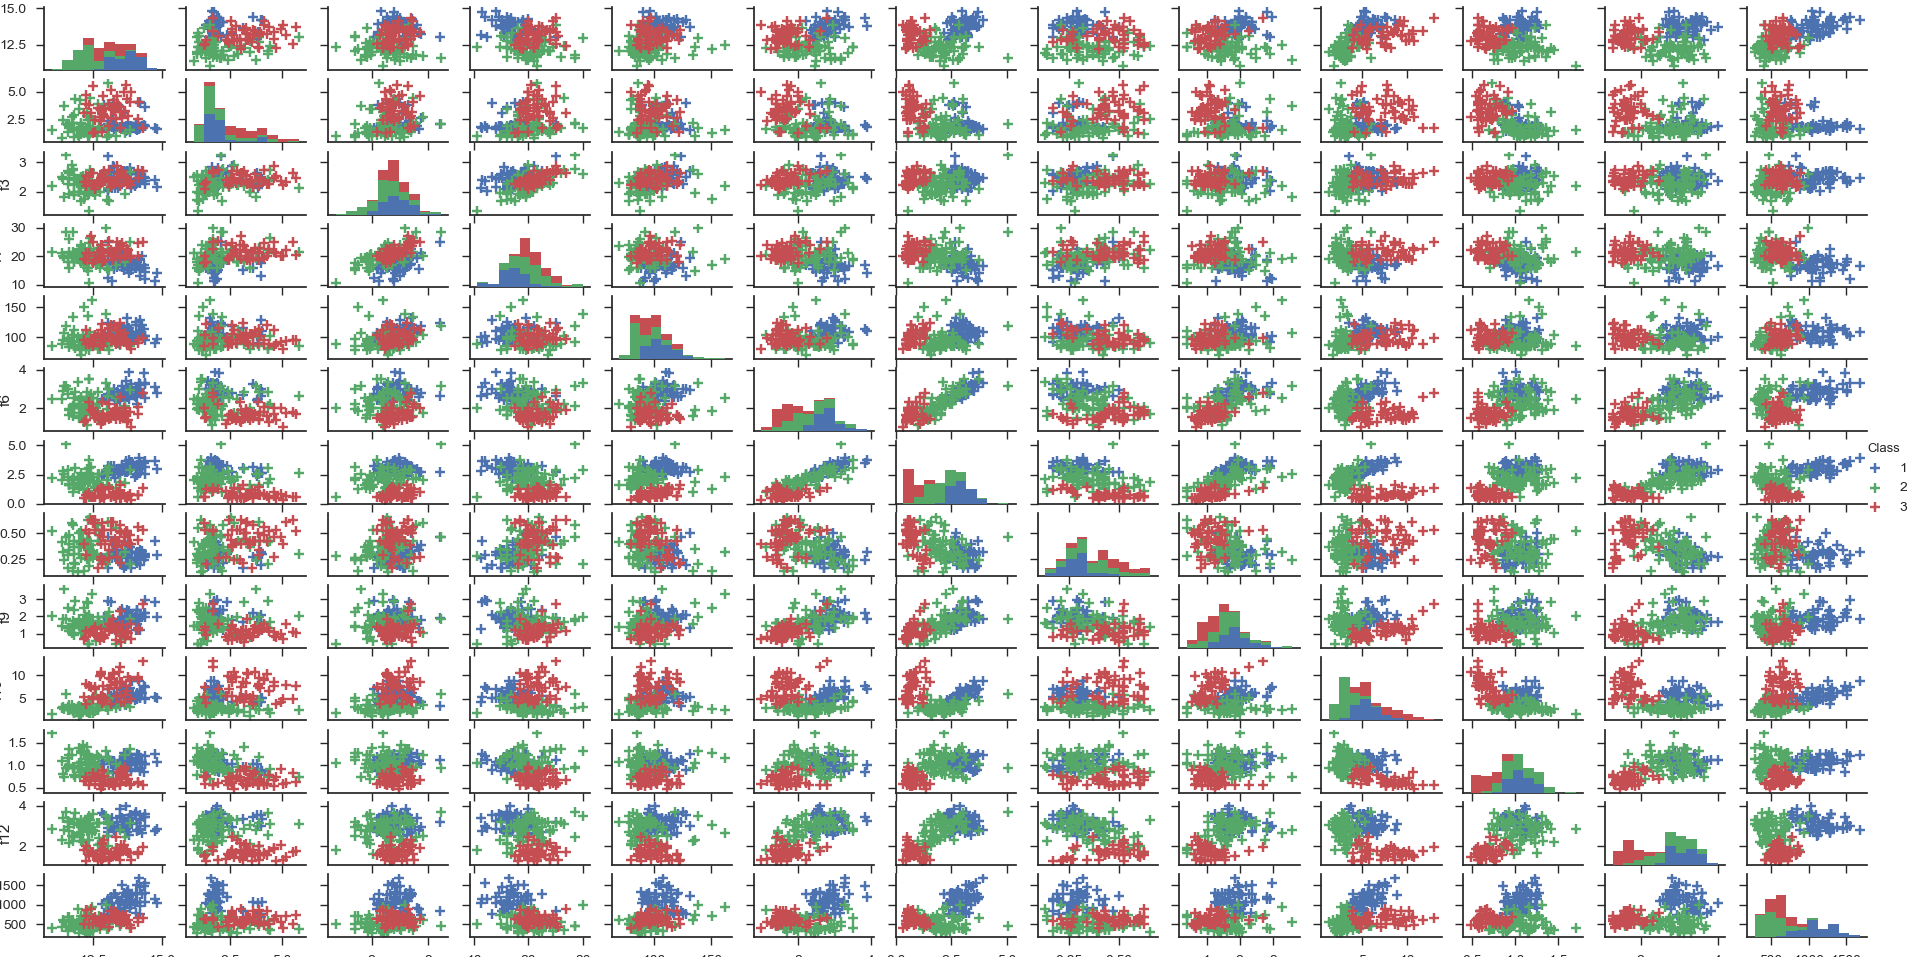
\includegraphics[width=1\textwidth]{dsWineCombined.png}
\caption{Rozkład cech dla zbioru Wine}
\end{figure}

\section{Metody klasteryzacji}
Zbadane zostaną dwie metody klasteryzacji.\\
\textbf{K-means}\\
Metoda ta polega na przyporządkowaniu danych wejściowych, w których każda próbka należy do klastra z najbliższą wartością średnią. Każda próbka to wielowymiarowy wektor liczb rzeczywistych.\\
Na wejściu algorytmu podawane są parametry : \\
k - ilość klastrów\\
data - dane wejściowe\\
Algorytm działa następująco:\\
1. Rozmieszcza centroidy  w losowych miejscach przestrzeni, \\
2. Dla każdego punktu znajduje najbliższą centroidę i przypisuje punkt do centroidy,\\
3. Na podstawie wszystkich próbek przypisanych do centroidy wyliczane są wartości średnie i powtarzany jest krok 2 dopóki warunki stopu nie zostaną spełnione lub nie nie zmieniło się przypisanie próbek.\\
Metoda przeznaczona jest jedynie dla danych numerycznych.\\
W funkcji klasteryzacji kmeans w R możemy zdefiniować maksymalną liczbę iteracji (domyślnie 10) oraz ilość losowań początkowych pozycji, z których wybrana zostanie najlepsza.\\
\textbf{Partitioning Around Medoids}\\
Używa ona zachłannego algorytmu, więc może nie znaleźć najlepszego rozwiązania, ale dzięki temu jest relatywnie szybka. Działa według następującego schematu.\\
1. Wybiera k reprezentatów, które będą centami klastrów.
2. Przypisuje wszystkie punkty do najbliższego klastra.
3. Dla każdej próbki będącą centrum medoidy i dla każdej próbki nie będącej centrum zamień je. Jeżeli konfiguracja pogorszyła się, cofnij zmianę.\\
Koszt wyliczany jest jako suma odległości próbek w klastrze od jego centrum.


\section{Ocena klasteryzacji}
Do oceny jakości klasteryzacji posłużą nam następujące miary:\\
\textbf{Purity}\\
Informuje w jakim stopniu klastry odpowiadają pojedynczym klasom. Warto zaznaczyć, że w przypadku takiej samej ilości klas co klastrów funkcja zawsze zwróci wartość 1.

$$ \frac{1}{N} = \sum_{m \in M} \max_{d \in D} | m \cap d |   $$

\textbf{Rand measure}
Porównuje jak podobne są klastry względem wzorca. Miara może być interpretowana jako procentowa ilość podjętych prawidłowych decyzji.

$$ RI = \frac{TP + TN}{TP + FP + FN + TN}$$

\textbf{Dunn index}
Miara ta odzwierciedla gęstość i poprawność odseparowania klastrów. Wyliczana jest na podstawie stosunku minimalnej odległości wewnątrz klastra do maksymalnej odległości wewnątrz klastra.

\textbf{Davies–Bouldin index}
Miarę tę można obliczyć na podstawie poniższego wzoru.

$$ DB = \frac{1}{n} \sum_{i=1}^{n} \max{(\frac{\sigma _{i} + \sigma _{j}}{d(c_i, c_j)})}   $$

Gdzie n jest liczbą klastrów, c - centroidą klastra, $ \sigma $ - średnia odległość od wszystkich elementów klastra. Algorytm dające niskie odległości wewnątrz klastra będą i duże odległości między klastrami będą dawały niskie wyniki.

$$  \hat{y} = arg \max_{y} P(y) \prod_{i=1}^{n} P(x_{i} \mid y) $$

$$ P(y\mid x_{1},..., x_{n}) = 
\frac
{P(y)P(x_{1},...x_{n}\mid y)}
{P(x_{1},...,x_{n})}
$$

\end{document}